\section{Vision}

Although the main intent of the vision was to detect the given set of objects (see figure \ref{fig:object_set},
it was later on also used to exploit wall and ground information for mapping and localization functionality.

\begin{figure}
\begin{center}
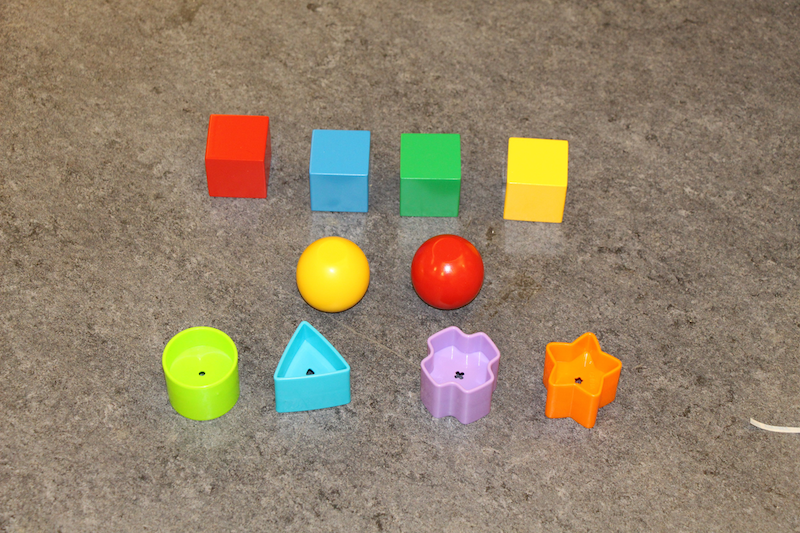
\includegraphics[width=0.38\textwidth]{figures/object_dataset}
\end{center}
\caption{Object data set}
\label{fig:object_set}
\end{figure}

\subsection{Object detection}

It was decided upon using the 3D information from the primesense to reduce susceptibility to illumination changes and to gain more information about the structure of objects.
Processing of the point cloud is mostly done with using the library \textit{Point Cloud Library}.
The detection and recognition can be divided in 4 different steps (see figure \ref{fig:vision:obj_det}).

\begin{itemize}
\item \textbf{Calibration:}
Takes the ground plane from the segmented planes and calculates the camera pitch and height.

\item \textbf{Transformation and subsampling:}
Receives a calibration matrix from the calibration and transforms the point cloud accordingly.
Simultaneously it downsamples the point cloud to reduce the number of points and so increase the processing speed in later steps.

\item \textbf{Plane segmentation:}
Takes in the subsampled point cloud and downsamples it even further so that only 1500 points are left.
Instead of using the regular approach of using voxel grid downsampling, offered by the PCL library,
the downsampling is performed by randomly picking 1500 points.
This is sufficient to have enough features on the planes.
RANSAC is applied to find all planes, until only a fraction of points is left unclassified (see result in figure \ref{fig:vision:seg_planes}).
To make use of the planes in mapping this step also calculates the oriented bounding box that the points on the plane encompasses.
Because two walls can lie on the same plane, a cluster segmentation is necessary to make the distinction.
The embedded euclidean cluster extraction turned out to be very expensive.
It was therefore decided to implement a 1D cluster segmentation. 
This can be achieved by projecting all points on the orthogonal vector of the planes normal vector, sorting them and finding gaps.

\item \textbf{ROI extraction:}
Takes in the segmented planes and removes all points in the point cloud that lie on that plane with regard to some distance threshold.
Euclidean cluster extraction, as implemented in the PCL library is applied to find clusters. 
Clusters that contain points lieing outside a given distance to the ground plane are immidiately dismissed.
The remaining clusters define the regions of interests (ROIs) and can be used for further processing.
\end{itemize}

\begin{figure}
\centering
\begin{subfigure}[b]{1.0\textwidth}
\centering
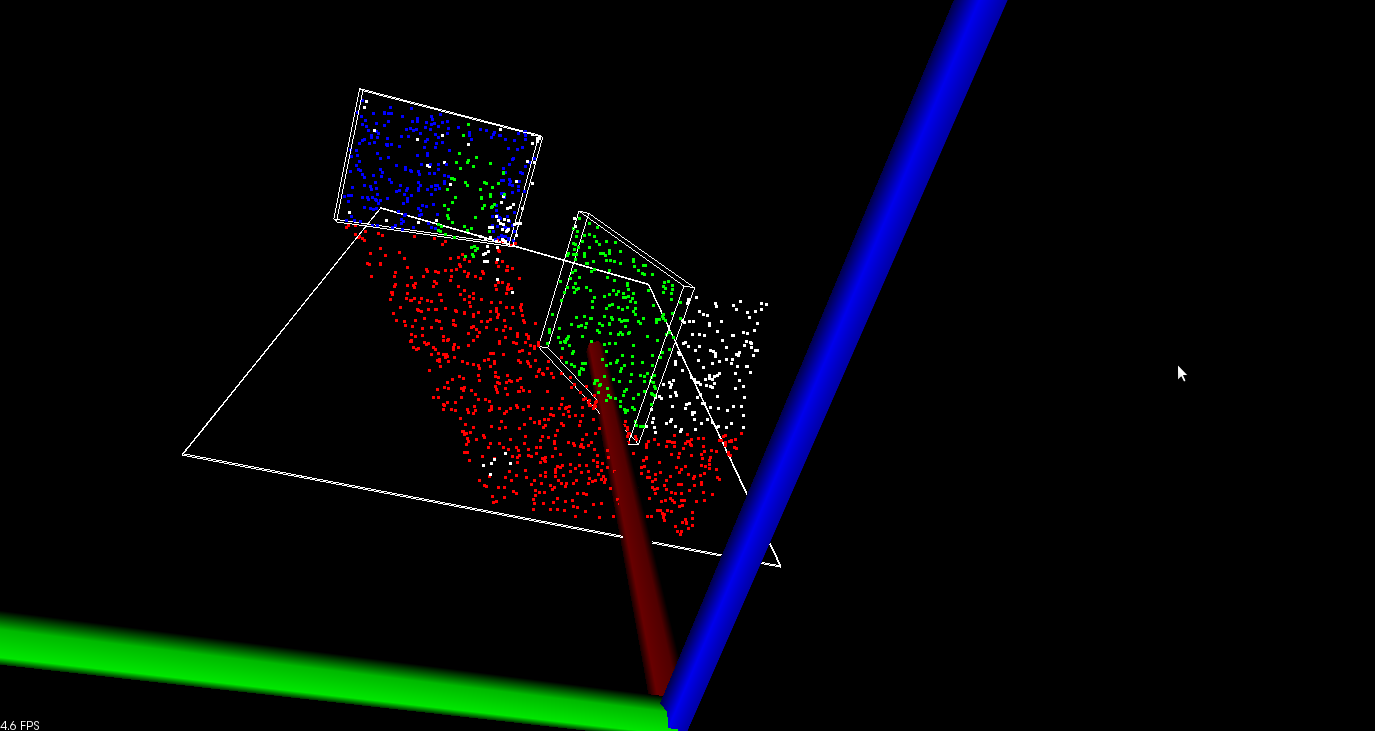
\includegraphics[width=0.8\textwidth]{figures/vision_planes.png}
\caption{Segmented planes. \textbf{Green:} Case when two unconnected walls are interpreted as one plane. Only the largest part is taken. \textbf{White:} Non segmented points.}
\label{fig:vision:seg_planes}
\vspace{10pt}
\end{subfigure}
\begin{subfigure}[b]{1.0\textwidth}
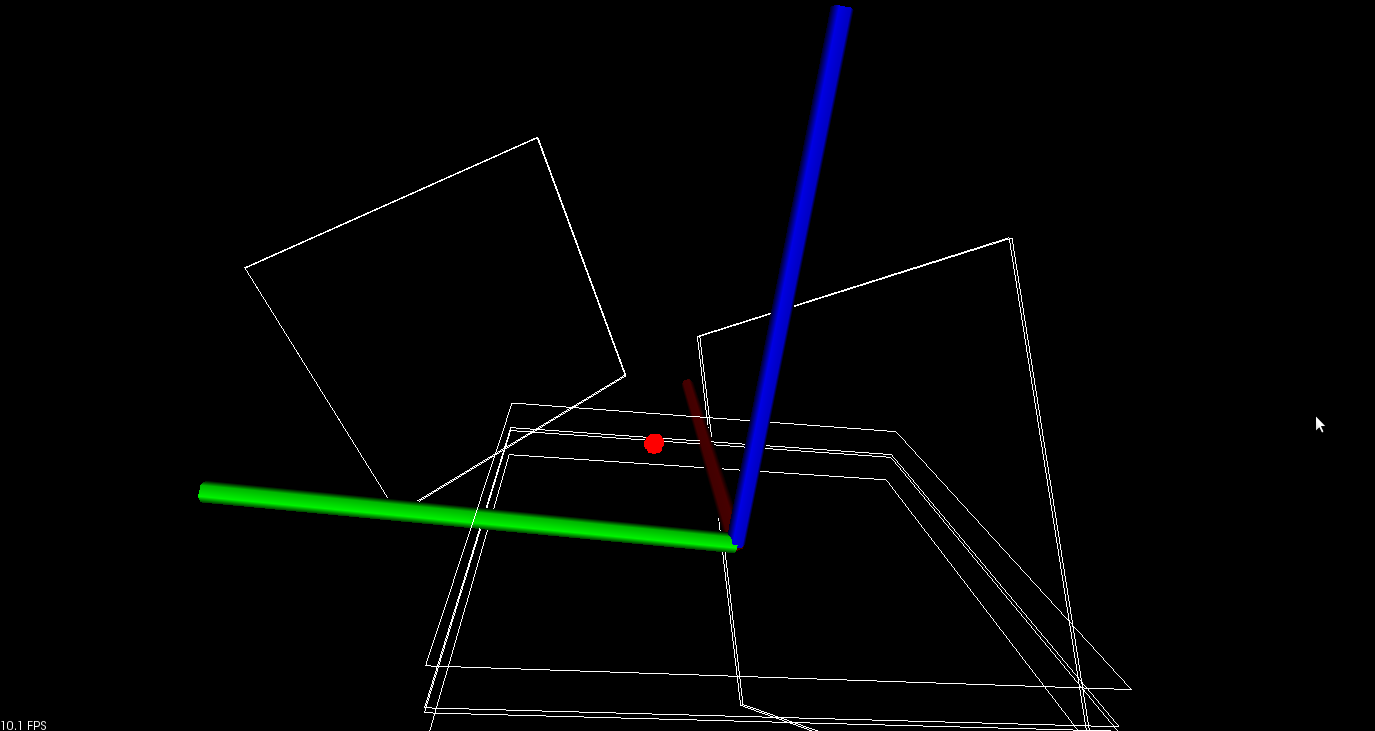
\includegraphics[width=0.8\textwidth]{figures/vision_roi_ball.png}
\centering
\caption{Segmented regions of interest. \textbf{Red:} ROI of a sphere. \textbf{Skewed rectangles:} Planes from (a). \textbf{Bottom sandwich:} Ground plane and maximum distance for accepting a cluster as a region of interest.}
\label{fig:vision:seg_rois}
\end{subfigure}
\caption{Results of the object detection}

\end{figure}

\begin{figure}
\centering

\begin{subfigure}[b]{0.49\textwidth}
\centering
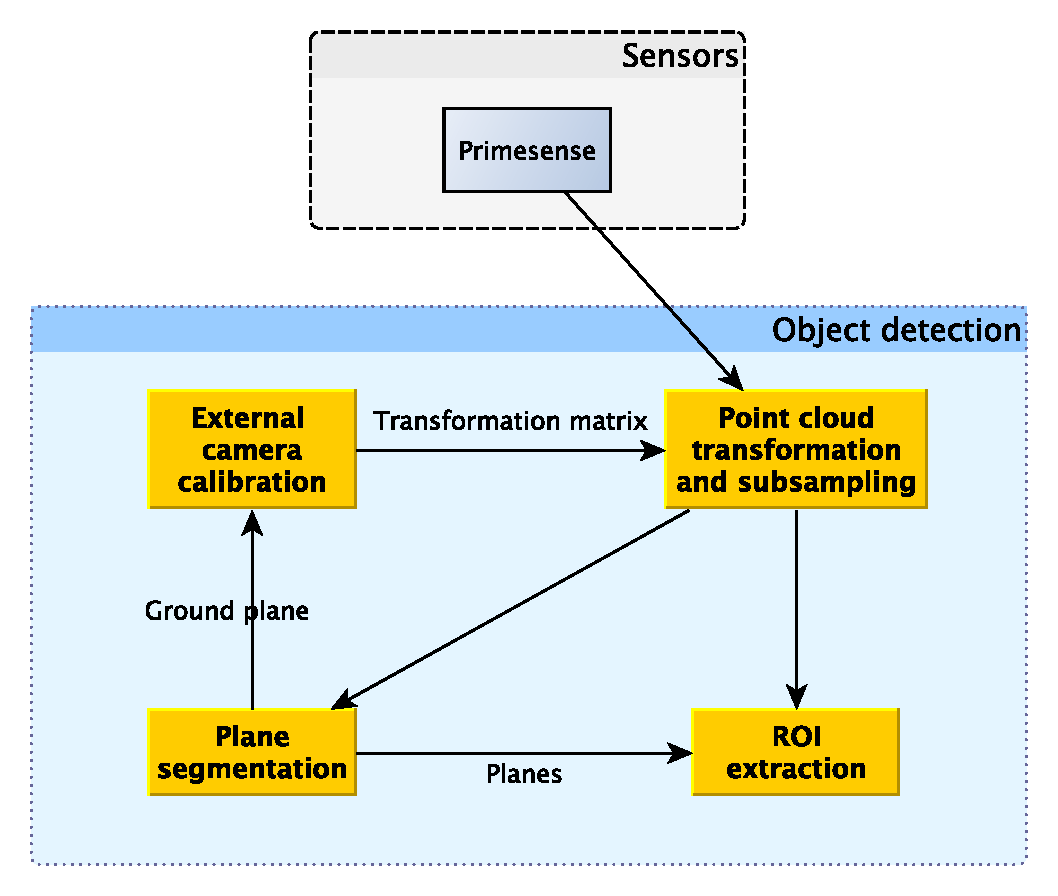
\includegraphics[width=\textwidth]{figures/arch_vision_obj_det.pdf}
\caption{Object detection}
\label{fig:vision:obj_det}
\end{subfigure}
%\hfill 
\begin{subfigure}[b]{0.49\textwidth}
\centering
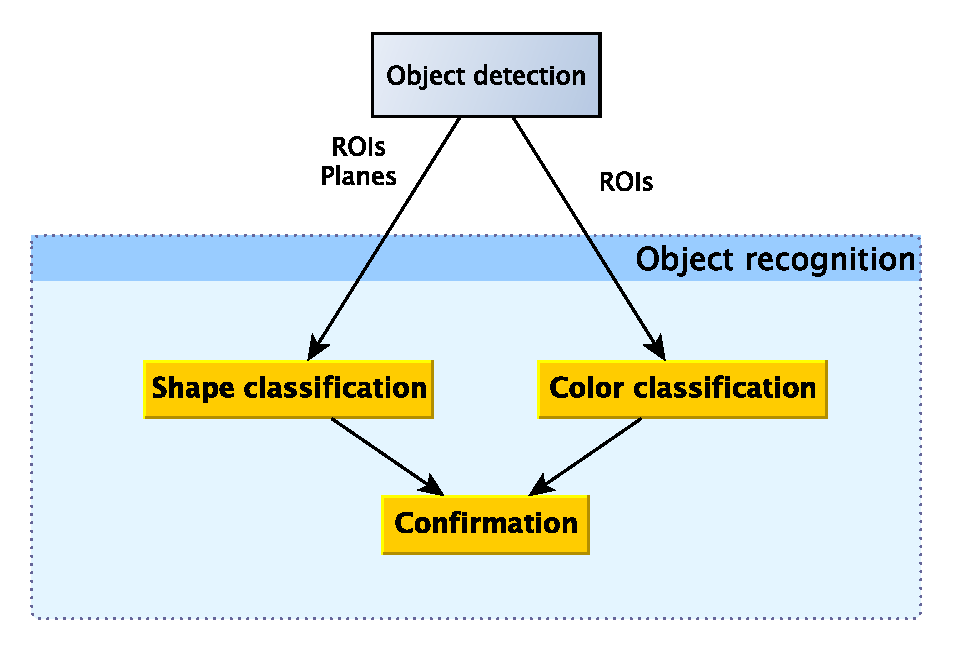
\includegraphics[width=\textwidth]{figures/arch_vision_obj_rec.pdf}
\caption{Object recognition}
\label{fig:vision:obj_rec}
\end{subfigure}
\caption{Vision - Process flow}
\end{figure}


\subsection{Object recognition} 
 
The object recognition consists of three phases itself (see figure \ref{fig:vision:obj_rec}).

\subsubsection{Shape classification}

Regarding shape classification, it relies mainly on exploiting the topology of the points lieing in the ROIs.
Three different shapes can be classified by applying different settings of RANSAC:
\begin{itemize}
\item \textbf{Spheres:}
Normals are estimated and RANSAC with model Sphere is applied.

\item \textbf{Cylinders:}
Normals are estimated and RANSAC with model Cylinder is applied.

\item \textbf{Cubes:}
RANSAC with model Plane is applied to exhaust all planes.
Multiple conditions are checked to verify that the planes describe a cube.
They mostly involve checks for perpendicularity regarding the ground and other planes.

\end{itemize}

All the other shapes can not be reasonably detected with RANSAC.
The major problem with those shapes though, is the generated point cloud by the Primesense.
Due to the whole in the top and bottom, the logic of the Primesense can not generate points especially around the region of the whole,
rendering the extracted clusters in the ROI extractor very small. 
Therefore they are often filtered out for being classified as noise.

\subsubsection{Color classification}

The color information is extracted from the point cloud which carries RGB information for each point.
Because color is highly susceptible to illumination changes, the perceived color can vary dramatically.
This makes it hard to obtain a robust but consistent color classification algorithm.

The analysis is made per color possible and not all at once, even though the algorithm is the same whatever the color.
We started by analising the HSV (hue, saturation, value) values we got from the regions of interest, mainly the hue, which is what defines the color. 
We then tried to find meaning in those values, mainly their average.
We concluded that for the most part, the overall average of hues of all the points in the region of interest would be enough to obtain a good estimate of the color. 
So we defined an area of each mean color value around which the color will be.
The bigger the margin, the more robust the algorithm would be.
However, because of the specific colors, the margin could not be too large, or the added robustness would not be reliable, as colors would start to mix.
Because different conditions may lead to very different results, we weighted two times the previous result based on specific situations, mainly, the percentage of points that have the color being tested relative to the total number of points, and the probability of being of the color being analysed, i.e., considering the point clouds don't usually have that many points, we give a higher weight to probabilities above a certain value.
Because the blob of interest may have points not only belonging to the object we want, but also from the ground or wall (if the object is very close to one), the number of points that have a color similar to orange, color of the ground, is also relevant in deciding the true color of the object, and hence helps in determining the weight of the probability of the color being analysed.
The end result is a somewhat robust algorithm and consistent as far as our testing went. 

\subsubsection{Confirmation}

To filter out false positives, a confirmation instance was added, that accumulates shape and color classifications over a specific time frame.
If a combination of shape and color occurred more often than others and it's ratio is greater than a threshold, it is returned as a confirmed classification.
Otherwise, if there is no classification for multiple frames whatsoever, the accumulation is reset.
